\chapter{Problemanalyse}
\textit{I dette kapitel analyses problemstillinger, som opstår i forbindelse med lægemiddelskift. Disse problemstillinger vil sammenfattes i en opsummering og afsluttes med en problemformulering, der fremadrettet danner  grundlaget for rapporten.}

\section{Lægemiddelskift}
Lægemiddelskift forekommer når en ny lægemiddelvirksomhed vinder leverancen af nyt lægemiddel som standardbehandling, hvormed der er indgås et kontraktskift~\citep{Amgros2015}. 

Forinden et kontraktskift kan forekomme analyseres og vurderes lægemidlet i samarbejde med Medicinrådet og Amgros~\citep{DanskeRegioner2016}, som beskrevet i Appendiks \ref{cha:AppA}. Efter analyseringen og vurdering sendes lægemidlerne i udbud via Amgros med henblik på at indkøbe lægemidler af høj kvalitet til bedst mulige pris~\citep{Sygehusapoteket2017}.

Størstedelen af lægemidler i ATC-grupper sendes i udbud en gang årligt fra start september til midt november, hvor udbud på ATC-grupper som indgår i Medicinrådets behandlingsvejledninger sker løbende hen over året~\citep{Sygehusapoteket2017}, som beskrevet i Appendiks \ref{cha:AppD}.
Forinden udbuddet defineres antallet af vindere samt, hvorvidt udbuddet skal bygge på laveste pris eller være mest økonomisk fordelagtigt~\citep{Amgros2018a}, som beskrevet i Appendiks \ref{cha:AppB}.

På baggrund af de foregående analyser og vurderinger fastsættes et prisniveau der anvendes som beslutningsgrundlag for Medicinrådet om, hvorvidt lægemidlet skal anvendes som standardbehandling~\citep{DanskeRegioner2016}. Hvis standardbehandlingen er det eneste lægemiddel inden for terapiområdet kan dette implementeres direkte på hospitalet. I tilfælde af flere lægemidler inden for samme terapiområde, skal lægemidlernes ligeværdighed vurderes af Medicinrådet, som beskrevet i Appendiks \ref{cha:AppA}, med henblik på at udarbejde behandlingsvejledninger og rekommendationer for lægemidlerne. Disse videresendes til de danske hospitaler, som står for implementeringen.~\citep{DanskeRegioner2016}

Kontraktskift medfører substitution af lægemidler, hvor et lægemiddel udskiftes til et andet~\citep{DanskSelskabforPatientsikkerhed2009}. Der findes to typer af substitution herunder analog og generisk.
Analog substitution omhandler lægemidler der indeholder forskelligt aktivt lægemiddelstof, har nogenlunde ens effekt og bivirkninger. Disse kræver ændring i ordination og skal derfor ordineret af en læge. Generisk substitution omhandler lægemidler som indeholder det samme virksomme lægemiddelstof og fungere derfor som hinandens synonyme. Dette skift kræver ikke en ændring i recept og kan derfor varetages af en sygeplejerske.~\citep{DanskSelskabforPatientsikkerhed2009}

Et simpelt lægemiddelskift er vurderet til at påvirke hospitalsafdelingen i lav grad og varetages logistik afdeling~\citep{Laegemiddelinformaion2017, Sygehusapoteket2017a}. Disse skift sker dagligt i forbindelse med et simpel generisk lægemiddelskift. Hvorimod et kompleks lægemiddelskift påvirker klinikken i mellem til høj grad og kræver ofte involvering af flere interessenter som f.eks. medicinansvarlig, overlæger, kontaktsygeplejersker eller medicinservicefarmakonomer til at undersøge lægemidlets anvendelighed for det pågældende hospitalsafsnit. 
De komplekse skift sker ved generiske lægemidler, hvor flere faktorer som f.eks. styrke og disponeringsform afviger fra den nuværende behandling.~\citep{Laegemiddelinformaion2017,Sygehusapoteket2017a}

\section{Problemstillinger ved lægemiddelskift}
Substitution af lægemidler kan medføre patientsikkerhedsmæssige konsekvenser~\citep{DanskSelskabforPatientsikkerhed2009}. Et norsk studie har undersøgt konsekvenserne ved generisk substitution~\citep{Hakonsen2010}. Interview med 100 sygeplejersker påviste at der opstod fejlmedicinering ved generiske lægemidler~\citep{Hakonsen2010}. Ud af disse følte 92~\% af sygeplejerskerne at generiske lægemidler var tidskrævende og 91~\% at risikoen for fejl øges ved disponering, hvoraf 42~\% havde oplevede fejl som følge af generisk substitution~\citep{Hakonsen2010}.
Medicineringsfejl ved generisk substitution fremgår af Figur \ref{fig:GeneriskSubstitution}.

\begin{figure}[H]\centering	\includegraphics[width=1\textwidth]{billeder/GenSub.png} 
	\caption{Medicineringsfejl ved generisk substitution rapporteret (n=100)~\citep{Hakonsen2010}.}
	\label{fig:GeneriskSubstitution}  
\end{figure}

Det fremgår af Figur \ref{fig:GeneriskSubstitution} at størstedelen af fejlmedicinering ved generisk substitution skyldes forkert lægemiddel, hvor en mindre del skyldes forkert formulering og i sjældnere tilfælde forkert dosis, administrationsvej og udeladelse af dosis. Yderligere blev årsager til fejlmedicinering rapporteret af 42 sygeplejersker~\citep{Hakonsen2010} og fremgår af Figur \ref{fig:GeneriskSubstitution1}.

\begin{figure}[H]\centering	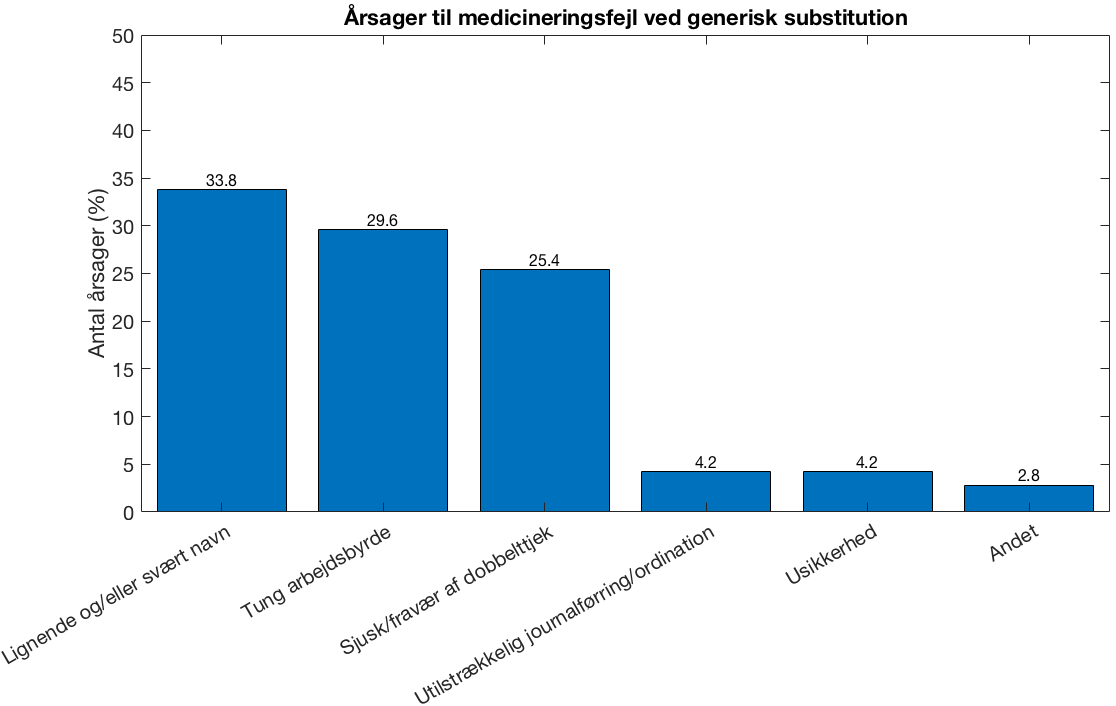
\includegraphics[width=1\textwidth]{billeder/GenSub1.png} 
	\caption{Årsager til medicineringsfejl ved generisk substitution (n=42)~\citep{Hakonsen2010}.}	\label{fig:GeneriskSubstitution1}  
\end{figure}

Af Figur \ref{fig:GeneriskSubstitution1} fremgår det at størstedelen af årsagerne til medicineringsfejl ved generisk substitution skyldes lignende og/eller vanskeligt lægemiddelnavn, kraftig arbejdsbyrde og sløvhed eller fravær af dobbelttjek. En mindre del skyldes utilstrækkeligt lægeattest og/eller recept, usikkerhed eller andet der kan være årsag til medicineringsfejl. 

I flere lande, inklusiv Danmark, opstår forkert lægemiddel ofte i forbindelse med forvirring ved  forveksling af navn eller emballage~\citep{DanskSelskabforPatientsikkerhed2009}, hvilket afspejles i det norske studie. Et eksempel på forveksling af navn er panodil, som er et smertestillende, og plendil, som anvendes til behandling af forhøjet blodtryk. Derudover kan disse fejl forekomme som følge af lægemidler med, uden eller forskellige suffix/præfix, som f.eks. Efexor kontra Efexor Depot, Levemir penfill kontra Levemir flexpen, hvilket kan give anledning til udlevering af et forkert lægemiddel.~\citep{DanskSelskabforPatientsikkerhed2009}

Yderligere angav nogle sygeplejersker at forvirringen over at finde det korrekte substitution medvirket til at de glemte alt om dosering og formulation. Forveksling af lægemiddelnavne har i sjældnere tilfælde haft konsekvenser som har medført forlænget indlæggelse, forværret sygdom eller dødsfald.~\citep{DanskSelskabforPatientsikkerhed2009}


Den tunge arbejdsbyrde.......skydels....

I forhold til sjusk og fravær af dobbelttjek blev det rapporteret af 27~\% sygeplejersker at det var kutyme at en anden sygeplejerske dobbelttjekkede før medicinen blev givet til patienten. Yderligere angav 48~\% at dobbelttjek kun skete i de tilfælde hvor de var usikre over situation. 

\section{Forebyggelse af problemstillinger ved lægemiddelskift}
Den europæiske lægemiddelstyrelse har udviklet guidelines med henblik på at forebygge problemer opstået ved forveksling af lægemidler og derved reducere antallet af medicineringsfejl~\citep{DanskSelskabforPatientsikkerhed2009}. Disse guidlines er ikke indført i Danmark, men der har været fokus på problemer med emballage forvekslinger, hvormed lovgivningen i Danmark er at pakninger ikke må kunne forveksles.   

Udover guidelines har internationle studier påvist at stregkode teknologi reducerer antallet af fejl i medicineringsprocessen~\citep{Poon2006, Levtzion-korach2010} Stregkode teknologi kan anvendes til at sikre at den rette medicin modtages af den rette patient~\citep{Amgros2013}.  
Amgros har siden år 2010 stillet krav til stregkode på yderste og inderste emballage på lægemidler~\citep{Amgros2013}. Foruden at undgå alvorlige medicinrelaterede fejl kan stregkoder medfører en mere enkel og sikker registrering af lægemiddel i patienternes medicinjournal og effektiv tilbagekaldelse af medicin via it-systemer~\citep{Amgros2013}. Implementering af stregkode teknologi er påvirket af manglende stregkoder og dokumentation ved generisk lægemiddel~\citep{Amgros2013}.

Det anbefales yderligere at anvende store og små bogstaver til navne på lægemidlerne i flere lande med henblik på at advare sundhedspersonalet om lignende lægemidler~\citep{ISMP2011,HQSC2013,ACSQ2011}. Sundhedspersonalet vurderede at det vil have en gavnlig effekt at blive advaret via Tall Man Lettering og at dette især vil have en betydning for lægemidler, hvor navneforveksling kan opstå~\citep{Campmans2018}.

Ligeledes har klinisk besluningstøtte i forhold til advarsler ved forveksling af navn og styrke vist sig at have en positiv effektiv i forhold til at forebygge antallet af medicineringsfejl~\citep{Campmans2018}. Flere studier har påvist at implementering af elektronisk beslutningsstøtte reducerer antallet af fejl~\citep{DW1998,Bates2013,Cheng2011,Raboel2005} og beskrives som et vigtigt redskab til at øge kvaliteten af medicinering med henblik på at nedbringe fejl~\citep{Raboel2005}. Klinisk beslutningsstøtte er anvendt i vid udstrækning inden for sundhedssektoren som f.eks. ved kontrol af lægemiddelallergier og interaktioner mellem to eller flere lægemidler~\citep{Raboel2005}. 

\section{Problemafgræsning}
På trods af at lægemidlerne sendes i udbud via Amgros med henblik på at opnå økonomiske besparelser er sundhedsudgifter til sygehusmedicin stigende~\citep{Sundhed2016,Sygehusapoteket2017}. Udover det økonomiske aspekt medvirker implementeringen af lægemiddelskift til patientsikkerhedsmæssige konsekvenser på grund af medicineringsfejl~\citep{DanskSelskabforPatientsikkerhed2009,Hakonsen2010}. Størstedelen af fejlene forekommer ved forkert lægemiddel ved generisk substitution og de hyppigeste årsager til dette skyldes lignende og/eller svært navn på lægemidlet~\citep{Hakonsen2010}. Guidelines er udviklet med henblik på at undgå forveksling af navn samt emballage på lægemidlerne~\citep{DanskSelskabforPatientsikkerhed2009}. Stregkode teknologier har påvist at have gavnlige effekter ved at reducere antallet af medicineringsfejl~\citep{Poon2006, Levtzion-korach2010}. Ligeledes er klinisk beslutningssøtte, som er anvendt i vid udstrækning inden for sundhedssektoren, påvist i flere studier at medvirke til reduceringen af fejl og anses samtidig som et vigtigt redskab til at øge kvaliteten ved medicinering~\citep{DW1998,Bates2013,Cheng2011,Raboel2005}.

\section{Problemformulering}
\textit{Hvilket potentiale har en algoritme som beslutningsstøttesystem til kategorisering af lægemidler med henblik på at forebygge fejl ved medicinering?}
